\todo{Dont start so heavy. Introduce the system first. Explain it after. Illustrate in the end}

The proposed system consists of a web application, composed of both a client, and server side application,
which are mutual exclusive but dependent upon another.
The basic structure and data flow of the proposed application is 
presented in figure \ref{fig:system_architecture_design}, which will 
be explained with further detail.


\begin{figure}[htpb]
  \centering
  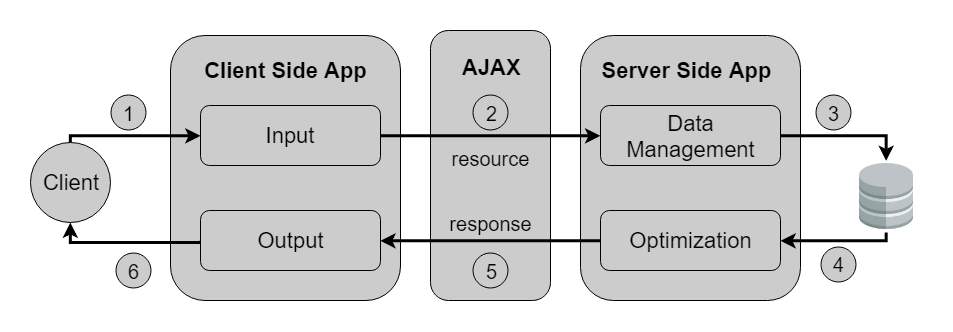
\includegraphics[width=\textwidth]{./Figures/system_design/system_architecture_design.png}
	\caption{Structure and data flow of the proposed application}
  \label{fig:system_architecture_design}  
\end{figure}


The client side application (CSA) is designed to interact with the user,
enabling the construction of requests (number 1 in the figure), 
and the presentation of solutions to those requests (number 6).
\todo{The details of this design and implementation are covered in section x and y, respectively.)}

\todo{Add a line saying that step 4) optimization, is not necessary in some requests. For example, single and round flights can be trivially solved by aplying some filter criteria. However, for multi city requests, and as the number of cities to visit increase, this problemas becomes harder to solve. Thus, we need to move it to the server. As a consequence, the complexity of the client application is reduced, because it does not hnadle optimization, and its only goal becomes to be an I/O port, where the input comes from the user, and the output from the server.  }

Due to the nature of the constructed requests, which are Np-hard for unconstrained multi city requests,
the optimization process associated to it is computationally heavy.
Thus, the response to a request is not processed by the client side application,
but rather by an application which runs on the server. 

The communication between the client and the server applications  
is done via Asynchronous Javascript and XML (AJAX),
which means that upon submiting the request (number 2 in the figure),
the client can continue to interact with the application 
while the response is being prepared.

The server side application is responsible for producing a 
response to the user constructed requests.
(As covered in section x), the user requests can be transformed into a Traveling Salesman Problem instance.
However, upon the construction of the request, only the nodes (cities) of the TSP problem are specified,
while the arcs (flights) which connect those nodes, are not.
Thus, it is crucial to complete the TSP graph with real fligh data (number 3 in the figure).
(This essential step of accessing real flight data may be subject to much discussion,
and is covered with more detail in section X).
Having access to a complete TSP graph, it is possible to run an optimization algorithm (number 4),
which produces the solution to the user request.

Finally, when the response is ready (number 5),
the client application uses this information to update and re-render the page, presenting the result (number 6).
(This interaction between both applications is discussed with more detail in section z.)
